\documentclass{article}
\usepackage[utf8]{inputenc}

\title{TUGAS GEOFISIKA I}
\author{VICKY VERNANDO DASTA - 1403114682}
\date{April 2017}

\usepackage{natbib}
\usepackage{graphicx}
\usepackage{listings}
\usepackage{verbatim}


\begin{document}

\maketitle

\section{Pengukuran Gravitasi}

persamaan untuk menentukan besar gaya gravitasi pada benda dari jarak x dari pengamat 
dengan menganggap bentuk benda adalah spherical sempurna, besar gayagravitasi dari jarak x bisa diukur menggunakan persamaan:


$$G(x)=\frac{4}{3}{\pi}{\rho}{d^{3}}{(x^{2} + z_{0}^{2})^{-1}} $$


phi: 3.14

rho: 1000 

d: 2

Z0: 10


berikut listing code Python:

\begin{lstlisting}
import matplotlib.pyplot as plt

def grav(x):
    return (4/3)*3.14*1000*(2**3)*(((x**2)+(10)**2)**-1)

# array of integers from range -40 to 40
x = range(-40, 41)
# create array g and calculate each numbers in x using 
# function grav with list comprehension
g = [grav(x_) for x_ in x]
# plot g with respect to x
plt.plot(x, g)
# title for x plane
plt.xlabel('jarak (x)')
# title for y plane
plt.ylabel('nilai gravitasi')
# title for the plot
plt.title('grafik fungsi gravitasi g terhadap jarak x')
# show result
plt.show()
\end{lstlisting}



Listing code diatas menggunakan bahasa pemrograman Python 3 dan Maplotlib sebagai library plotting. Hasil plotting nya sebagai berikut:

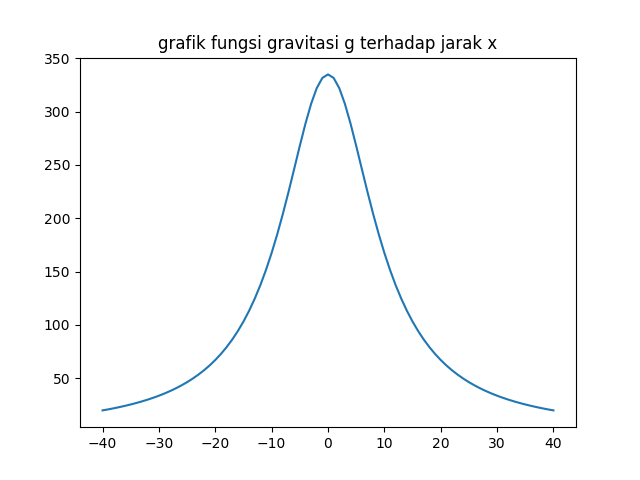
\includegraphics{plotgeo.png}

\section{Kontur Gravitasi}
``I always thought something was fundamentally wrong with the universe'' \citep{adams1995hitchhiker}

\bibliographystyle{plain}
\bibliography{references}
\end{document}
